\hypertarget{part-1-design-2}{
\section{Part 1, design 2}\label{part-1-design-2}}

\begin{figure}[ht]
  \centering
  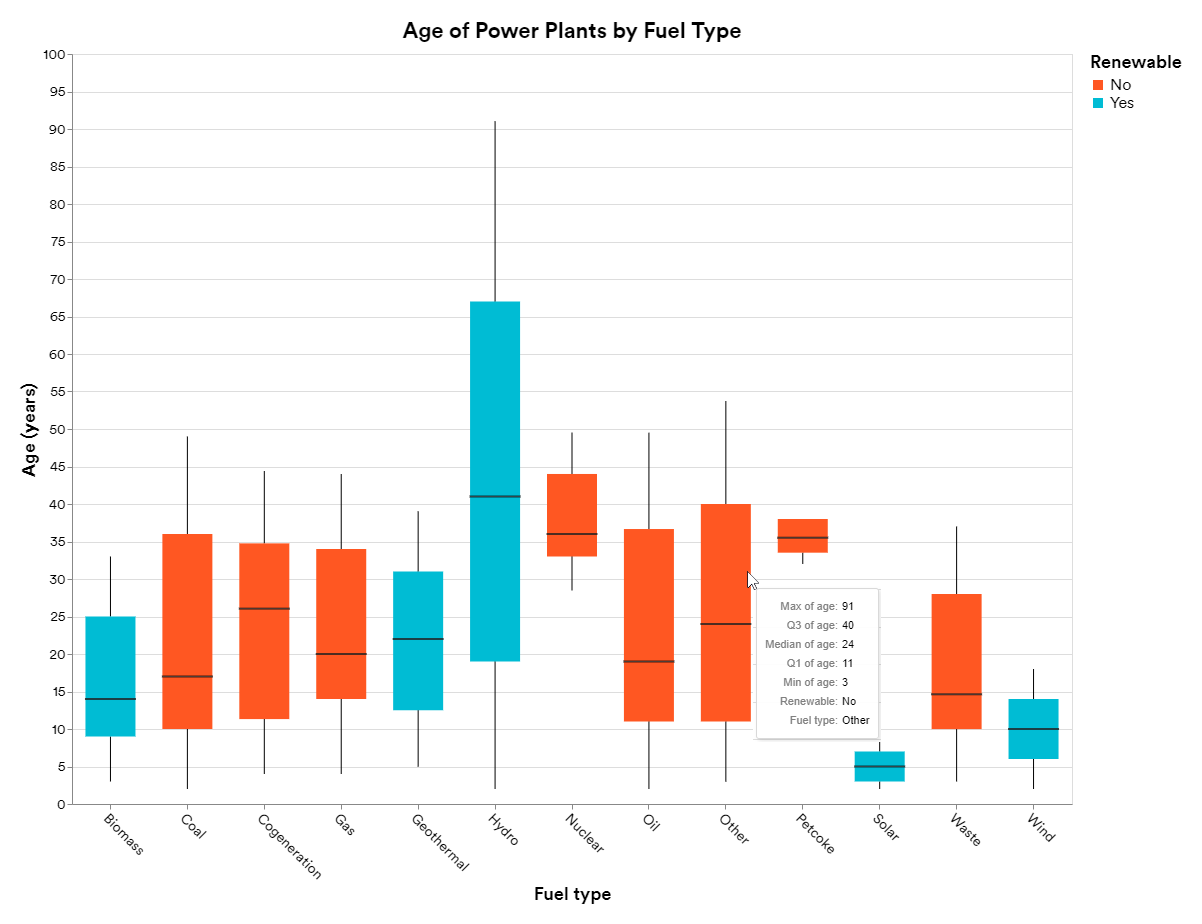
\includegraphics[width=\textwidth]{../img/design2}
  \caption{Age of power plants by fuel type (Design 2)}
\end{figure}

\hypertarget{description}{
\subsubsection{Description}\label{description}}

\begin{description}
\item[Visual Design Type:]
Box plot
\item[Name of Tool:]
Altair
\item[Country:]
Worldwide
\item[Year:]
N/A

\item[Visual Mappings:]
% each of the visual design mappings; include the data apping information about colour, shape, size, position (x/y axes), and any other visual mappings 
\begin{itemize}
  \item \textbf{Boxes}: The coloured boxes illstrate the variability, or spread (interquartile range) of the ages of each fuel type.
  \item \textbf{Whiskers}: A relative minimum and maximum power plant age for each fuel type is illustrated by the extent of the whiskers (vertical black lines).
  \item \textbf{Median}: The horizontal black line within each box indicates its median, or roughly the average age of power plants of each fuel type.
  \item \textbf{Hue}: The hue of a box is either blue or orange, indicating if the fuel type is renewable or non-renewable respectively.
  \item \textbf{Tooltip}: Tooltips are used to offer detail-on-demand to the user, showing precise information about the distribution of the ages.
\end{itemize}

\item[Unique Observation:]
% things we can learn from the visualisation e.g. from this vis we can see this pattern
Power plants have lifespans, and it is crucial to ensure that plants are as modern and efficient as they can be. This chart shows the general range of ages of power plants worldwide such that opportunities to enrich or update ageing plants can be identified, and also allows the user to keep an eye on emerging fuel types. We can easily identify that hydroelectric power plants have been the longest-running source of energy, and plants have been built regularly for most of hydro power's history.

The visualisation makes it plain to see the usage and evolution of fuel generation over the years, as the box plots highlight clearly the eras at which different fuel types were more prevalent. We see that highly-polluting petroleum coke plants were built mostly in a five-year period 35 years ago, whereas more modern fuels such as solar or wind have only been established in the last seven years or so. In fact, all renewable sources with the exception of hydro power have generally been built sooner than those non-renewable.

\item[Data Preparation:]
% any modifications to the original data that had to be performed to generate your beautiful image
This chart required only the provided GPPD data set, so preparation was minimal; age was calculated for each plant based on the year of commissioning, a simple query was used tell apart renewable and non-renewable sources.

Additionally, outliers have been hidden on the chart as they introduced almost random clutter with little meaning.

\end{description}

% Describe the insight that your visualizations provide. What can we learn from
% your visualizations? How are they better than a standard line, pie, or bar
% chart?